\documentclass[prd,nofootbib,floatfix,11pt,tightenlines,nofootinbib]{revtex4}
%\documentclass[useAMS,usenatbib,tightenlines,11pt,preprint]{aastex}
\usepackage[paperwidth=8.5in,paperheight=11in,centering,margin=1in]{geometry}

\usepackage{parskip}
%\setlength{\parskip}{\baselineskip}
\parskip=5pt

\usepackage{amsmath}
\usepackage{amsbsy}
\usepackage{squeeze}


\input epsf
\usepackage{amsmath,amssymb,subfigure}
\usepackage{graphicx}
\usepackage{epsfig}
\usepackage{color}
%\usepackage{ulem}
%\usepackage{epstopdf}

%commented out the line below to get rid of citations that run into margins
%\usepackage{multicol}

%\usepackage{etoolbox}

\pagestyle{empty}


\renewcommand{\baselinestretch}{0.99}

%%%%%%%%%%%%%%%%%%%%%%%%%%%%%%%%%%%%%%%%%%%%%%%%%%%%%%%%%%%%
%%%%%%%%%%%%%%%%%%%%%%%%%%%%%%%%%%%%%%%%%%%%%%%%%%%%%%%%%%%%
%%%%%%%%%%%%%%%%%%%%%%%%%%%%%%%%%%%%%%%%%%%%%%%%%%%%%%%%%%%%

\begin{document} 

\begin{center}
{\bf \Large Learning in an Era of Uncertainty}
\end{center}

\vspace{1cm}

\noindent
\begin{tabular}{ll}
{\bf Applicant/institution: } & University of Washington\\
{\bf Street Address: } & \\
{\bf Principal Investigator: } &Andrew Connolly \\
{\bf Telephone number: } & (206) 543 9541 \\
{\bf Email: } & ajc@astro.washington.edu \\
{\bf Administrative POC name:} & Lynnette Arias\\
{\bf Telephone number:} & 206-543-4043\\
{\bf Email:} & osp@uw.edu\\
{\bf Funding Opportunity FOA Number:} & DE-FOA-0000918 \\
{\bf DOE/OSP Office: } & Office of Advanced Scientific Computing Research \\
{\bf DOE/Technical Contact: } & Dr. Alexandra Landsberg \\
{\bf PAMS Preproposal tracking number: } & PRE-0000002147 \\
\end{tabular}

% \noindent 
% \begin{tabular}{ll}
% {\bf Applicant/institution: } & Carnegie Mellon University \\
% {\bf Street Address: } & 5000 Forbes Ave, Pittsburgh, PA  15213 \\
% {\bf Co-Principal Investigator: } & Jeff Schneider \\
% {\bf Telephone number: } & (412) 268 2339 \\
% {\bf Email: } & schneide@cs.cmu.edu \\
% {\bf Administrative POC name, number, email:} Kristen Jackson, (412) 268 9527, kristenr@andrew.cmu.edu & \\
% {\bf Funding Opportunity FOA Number:} & DE-FOA-0000918 \\
% {\bf DOE/OSP Office: } & Office of Advanced Scientific Computing Research \\
% {\bf DOE/Technical Contact: } & Dr. Alexandra Landsberg \\
% {\bf PAMS Preproposal tracking number: } & PRE-0000002147 \\
% \end{tabular}

\newpage

{\bf Collaborating Institutions:} \\
Lead Institution: University of Washington, PI Andrew Connolly \\
Collaborating Institution: Carnegie Mellon University, PI Jeff Schneider \\

{\bf Lead PI:} Andrew Connolly \\

\noindent
\begin{tabular}{|l|l|l|r|r|r|r|}
\hline
\multicolumn{7}{|c|}{\bf Learning in an Era of Uncertainty} \\ \hline
&       &             & Year 1 & Year 2 & Year 3 & Total \\
& Names & Institution & Budget & Budget & Budget & Budget \\ \hline
Lead PI & Andrew Connolly & U Washington & \$170K & \$170K & \$170K & \$510K \\ \hline
Co-PI & Jeff Schneider & Carnegie Mellon U & \$170K & \$170K & \$170K & \$510K \\ \hline
{TOTALS} & & & \$340K & \$340K & \$340K & \$1020K \\ \hline
\end{tabular}

% \label{firstpage}

% \maketitle 
\pagebreak

%\begin{center}
%{\bf \Large Learning in an Era of Uncertainty}
%\end{center}

\pagestyle{plain}
\setcounter{page}{1}

\section{Introduction}

A new generation of DOE sponsored data intensive experiments and surveys,
designed to address fundamental questions in physics, materials, and
biology will come on-line over the next decade. These experiments share
many similar challenges in the fields of statistics and machine-learning:
how do we choose the next experiment or observation to make in order that
we maximize our scientific returns; how do we identify anomalous sources
(that may be indicative of new events or potential systematics within our
experiments) from a continuous stream of data; how do we characterize and
classify correlations and events within data streams that are
inherently noisy and
incomplete. The goal of this proposal is to address these challenges
through the development of machine learning techniques that better quantify the
uncertainty in their predictions and corresponding active experiment
selection algorithms that utilize those uncertainties to get the most
scientific information out of limited data collection budgets.

{\it Active learning} algorithms iteratively decide which data
points they will collect outputs on and add to a training set.  Their
goal is to choose the points that will most improve the model being
learned.  At each step, they consider the current training data, the
potential data that might be obtained, and the current learned model,
and evaluate what would be the best choice for the next observation,
experiment, or feature such that it improves our knowledge of the
overall system (according to some objective criterion). The potential
impact of active learning algorithms is substantial (optimizing the
scientific returns from billion dollar investments in observational
facilities). To achieve these breakthroughs requires that we address
the challenge of how to scale active learning to the size and
complexity of the data expected from this next generation of
experiments.  For example, our inability to undertake a full look
ahead to the end of all possible experiments results in the
development of myopic heuristics that improve the speed of these
learning techniques but at a substantial cost in how well they perform
on real data.  See, for example, 
Figure 1 from reference \cite{Garnett11} and Figures
3 and 4 of reference \cite{Garnett12}.

By addressing these challenges we propose to develop active learning
algorithms that will scale to data sets with hundreds of millions of
entries and petabytes of data. This work has the potential to impact
many of the data intensive sciences. For this proposal, however, we
will focus our work in the context of DOE sponsored cosmology
experiments (i.e.\ the Dark Energy
Survey\footnote{http://www.darkenergysurvey.org}, and the Large
Synoptic Survey Telescope\footnote{http://www.lsst.org}). These
surveys are ideal proxies as their bandwidth (terabytes of data per
night and petabytes of data every couple of months) will enable high
precision studies of cosmology. The ability to use these data sets to
achieve an order of magnitude improvement in constraints on our
understanding of cosmology and dark energy will, however, depend on
how well we can analyze, optimize, and calibrate data streams that are
noisy and incomplete. This will require the development of
fundamentally new approaches to the analysis of data at a scale,
speed, and complexity beyond the capabilities of current automated
machine learning methods.

\subsection{Project Objectives}
\label{sec:objectives}

On-line, data-driven analysis will require model-fitting and
classifications that are non-parametric and probabilistic.  Gaussian
Processes (GPs) meet these requirements and we will, therefore, build our
methods around them.  We note, however, objectives 2-4 below will result in
algorithms that do not depend on this choice, and should be applicable to
any regression or classification method that yields a probability
distribution over outcomes.  We divide our research program into the
following objectives.

{\bf (1) Designing Robust Gaussian Processes.}  Applying GPs to the future
of big data science will require confronting problems not yet addressed by
automatic data analysis algorithms. Most model-fitting algorithms,
including GPs, return a prediction and an error on that value that is
unimodal and usually Gaussian.  As future experiments push the boundaries
of our physical understanding, this assumption will cease to be valid.  A
particularly difficult case is where the data allows multiple
interpretations and thus the real posterior belief about a variable should
be multi-modal.  We propose new methods that allow GPs to provide these
predictive distributions.  Experiments in high energy physics,
astrophysics, and biology are not only expensive, but are also sometimes
impossible in some regimes.  We need to make inferences across regimes
where training data is either very sparse or not available at all and
propose methods to do so in GPs.

{\bf (2) Active Learning.} Supervised regression and classification
algorithms require labeled data points for training.  These output labels
are typically assigned by human experts and/or additional data
collection.  Often, the resources required (both in terms of human-hours
and experimental apparatus) are considerable.  We propose to develop new
algorithms to optimize the use of these resources by determining what event
or object labels will maximize the improvement to models from supervised
learning algorithms.

{\bf (3) Active Feature Acquisition.}  Active learning selects specific
unknown events or objects for follow-up observation and classification by
human experts.  Active feature acquisition further refines the inquiry by
asking what kinds of follow-up observations will yield the most information
about the unknown object.  We will develop algorithms for this using
Gaussian processes.

{\bf (4) Active Search.} Often it is the anomalous events or objects from
rare classes within large streams of data that lead to fundamental
scientific breakthroughs. We, therefore, require methods that allocate most
observational resources to those objects.  This is an active search
problem. As in active learning, the acquisition of class labels is
expensive and we need to learn a model to predict these labels from limited
input data. The final performance objective is, however, not the accuracy
of the classifier, but rather the number of positives (i.e. objects from
interesting classes) observed.  We will develop algorithms that do active
search in combination with achieving the other objectives.

% We
%propose to use the simple myopic algorithm described in that work.  It
%computes the probability of each point belonging to the positive class and
%chooses the largest.



%The active search and active learning algorithms each compute an objective
%criterion score for each object.  For photometric redshifts the scores are
%used to create a ranked list and observations are scheduled proceeding down
%the list.  When a budget is given for follow-ups on each batch of newly
%detected transients, going down a ranked list in each batch until that
%budget is exhausted is appropriate.

%However, when the budget is an aggregate over a longer time period a
%streaming decision on how much of the budget to spend on each batch must be
%made on that batch in isolation.  This will be done by choosing a score
%threshold.  The threshold will be set by evaluating the historical stream
%and setting it at a value that would yield a number of follow ups equal to
%an available budget for following up.  The threshold will be adjusted
%continuously as more observations are taken and the models and scientific
%goals change (e.g. the object types designated as ``interesting'' are
%changed).

{\bf (5) Science Outcomes.}  Data from the Dark Energy Survey will become
publicly available over the term of this project (together with detailed
simulations of the expected data flow from the LSST).  We will, therefore,
use these data to demonstrate that the algorithms developed above will
improve the cosmological reach of the DES and LSST in the areas of improved
determination of photometric redshifts (see Section \ref{sec:photoz}) and
improved classification and online follow-up of transient sources (see Section \ref{sec:transients}).  We will release our software
publicly and seek collaborations where our algorithms may be spread to
other sciences -- such as climatology and microbiology -- wherein complex
systems can be modeled or measured at great expense and algorithms are
required to determine which models and experiments are actually worth
performing.

% Each of these goals will require us to develop algorithms to simultaneously
% learn the latent physical model underlying a given data set, the
% uncertainties around that model, and the potential information to be gained
% by futher studying a specific instance of the model (``event'' or
% ``object'').

\subsection{The Collaboration}

To accomplish the objectives laid out in this program we have
assembled a team experienced in algorithm design, data structures, and
in developing and delivering data mining algorithms that are actively
used by the cosmology community. The PIs of this research proposal
have a proven track record for propagating research ideas in
educational and multidisciplinary environments. Connolly and Schneider
have been part of an ongoing collaboration between machine learning,
cosmology and statistics for over a decade (noted by the President
of the American Statistical Association (ASA) as an exemplary
interdisciplinary research team \cite{straf03}).

Highlights from this collaboration include n-tree searching algorithms that
make the calculation of n-point correlation functions scale to the size of
current surveys \cite{GrayMoore} and that enable rapid characterization of
orbital tracks in sparsely sampled temporal data \cite{kubica}. The
software associated with these algorithms was made publicly available and
has been used to compute the 2--point function on over 10$^6$ galaxies and
the 3--point correlation function of 400,000 galaxies from the SDSS survey
\cite{Scranton2002,Szapudi2002,Nichol2006,mcbride2011a,mcbride2011b} as
well as in measures of the marked correlation functions \cite{Skibba2006}.
As part of this collaboration,
references \cite{yip2004a, vdp2009, daniel2011}
introduced to astrophysics signal compression and analysis techniques that
are now regularly applied to the analysis of spectroscopic surveys. More
recently this collaboration has developed algorithms for automatically
classifying astrophysical objects \cite{vdp2009,daniel2011} as well as an
initial set of papers that use a simplified active learning method to
accelerate the exploration of complex parameter spaces \cite{daniel2012}.
Schneider's group has led the development of new methods of regularization
to learn complex models with only a small amount of training data
\cite{YiZhangICML2010,YiZhangSDM2010,YiZhangMultitask2010,YiZhang2011multiECOC,YiZhang2012},
new non-parametric estimators for divergences and dependencies
\cite{poczos11alphadiv,Poczos2011UAI,poczos12CVPR}, and new graphical
models for finding groups of collectively anomalous records
\cite{Xiong2011gad,xiong2011fgm}.  Most recently, his group's work on
active search and active learning provides some starting points for the
proposed effort \cite{Tesch13,Wang13,Sutherland13,Garnett12}.
 
Connolly leads the University of Washington data management group that
develops the algorithms and techniques for the real-time analysis of
LSST data (including the detection and characterization of
transients and anomalies).  Schneider heads a machine learning group
that has done extensive work on automatic anomaly detection and
pattern-recognition in complex data sets
\cite{Xiong2011gad,poczos12CVPR}.  Schneider, and Connolly are members
of the Large Synoptic Survey Telescope collaboration with Connolly the
software coordinator for the DOE sponsored Dark Energy Science
Collaboration (a collaboration of over 150 scientists working on the
characterization of dark energy).


On the educational front, all PIs have developed and taught computational techniques at the
graduate and undergraduate level including data-mining for
Astrophysics. Connolly recently completed a text book ``Statistics,
Data Mining, and Machine Learning in Astronomy: A Practical Python
Guide for the Analysis of Survey Data'' that will be published by
Princeton University Press and provides a comprehensive introduction
to cutting-edge statistical methods together with the software
associated with these techniques. 
%On sabbatical at Google, Connolly led the
%development of Sky in Google Earth (aka Google Sky;
%http://earth.google.com/sky), which was similarly successful at
%engaging the public.
%
%We expect the proposed research to move beyond astrophysics to other
%data intensive sciences. In its broadest sense machine learning for
%massive Petabyte data archives drives many of the physical and
%biological sciences with catalogs containing hundreds millions of
%samples with thousands of measurements. The algorithms to be
%investigated here will also impact machine learning beyond their
%application to cosmology.  They move beyond the traditional learning
%of full models and are able to handle data that do not need to be
%pre-assembled into temporal sequences.  If successful, this will add
%new types of data sets and by inference new scientific fields to the
%list that can benefit from active learning of models.

\section{The Role of Active Learning in Cosmology}

Over the last decade a concordance model has emerged for the universe
that describes its energy content. The most significant contribution
to the energy budget today comes in the form of ``dark energy'', which
explains the observation that we reside in an accelerating
universe. Despite its importance to the formation and evolution of the
universe there is no compelling theory that explains the energy
density nor the properties of the dark energy. Understanding the
nature of dark energy remains as one of the most fundamental questions
in Physics today, impacting our understanding of cosmology, particle
physics, and potentially theories of gravity itself.  As noted in the 
report of the Dark Energy Task Force (DETF; constituted jointly by
DOE, NSF and NASA), ``the nature of dark energy ranks among the very
most compelling of all outstanding problems in physical science''.


To address the question of the nature of dark energy a new generation
of DOE sponsored experiments are entering service (e.g.\ the Dark
Energy Survey and the
Large Synoptic Survey Telescope).  These
surveys will represent a 40-fold increase in data rates over current
experiments (generating over 100 Petabytes of data over a period of 10
years) and decreasing the uncertainties on our measures of the
underlying properties of dark energy by more than a factor of ten.
At the scale of these experiment, statistical noise will no longer
determine the accuracy
 to which we can measure cosmological
parameters. The control and
 correction of systematics will
ultimately determine our final
 figure-of-merit. For example,
systematic errors in the estimation of cosmological distance or in the
identification and classification of high-energy transient events
(e.g. supernovae) lead to biases in the derived cosmological
parameters. A bias of just 1\% in distance (at a redshift $z=1$) degrades
measures of the properties of dark energy by over 50\%
\cite{kitching,huterer2006,nakajima2011}.

%\subsection{orphaned paragraphs about the importance of our science cases}
%
%The accurate determination of an object's distance or redshift is
%central to every test of cosmology that happens outside of a particle
%accelerator.  The comparison of redshifts and luminosities of standard
%candles enabled the discovery of dark energy and cosmic acceleration
%\cite{perlmutter1998}. Redshifts serve as a proxy for radial distance
%from Earth to the observed object.  Redshifts thus are necessary for
%building three dimensional maps of the distribution of galaxies in the
%Universe.  Such maps will help and have helped us to constrain how
%galaxies formed over the history of the Universe, and thus can tell us
%much about how gravity operates at the largest scales and what the
%parameters are that govern the behavior of dark energy, dark matter, 
%and the cosmic
%acceleration \cite{muvarpi2,roland,sudeep,linder2013}.  Accurately determining the redshifts of
%distant galaxies is a requirement if we are to answer some of the most
%vexing problems in fundamental physics today.
%
%Direct spectroscopic redshift measurements of enough galaxies to
%constrain dark energy parameters to the precision required by next
%generation experiments would be thousands of times more expensive than
%taking the corresponding photometric (or imaging) data.  Large digital
%cameras (e.g.\ the 3.2 Gigapixel camera for the LSST) can observe
%$\sim 10^6$ sources every 15 seconds (several orders of magnitude more
%efficient that spectroscopic observations). Our task, then, is to
%construct algorithms whereby we can convert these much cheaper
%photometric data into accurate redshifts (i.e. photometric redshifts).
%
%The demands of next generation cosmological experiments will require
%that our photometric redshift determinations be accurate to within
%$\le 2\times 10^{-3}(1+z)$ \cite{desc}.  This is a hard limit, as a
%bias in redshift determination of just 0.01 can degrade dark energy
%constraints by as much as 50\%
%\cite{kitching,huterer2006,nakajima2011}.  Testing present forward-fitting
%and empirical methods on a sample of 5,482 galaxies from the 2df-SDSS
%LRG and Quasar survey, Abdalla {\it et al}. (2011) find biases of
%order 0.05 (see their Figure 4).  This level of bias can degrade dark
%energy constraints by as much as a factor of 3 \cite{Ma2006}.
%Considering 3,000 galaxies from the DEEP2 EGS and zCOSMOS surveys and
%using Bayesian methods, Mandelbaum {\it et al}.  (2008) find a bias in
%redshift determination of order 0.01 (see their Table 2).  While this
%is an improvement, it still an order of magnitude larger than what is
%required.
%

\section{A Probabilistic Framework for Scientific Inference}

Current state-of-the art algorithms attempt to learn a 
model as a one-to-one
relationship between the input data and the output function. Uncertainties are
also learned, but these are usually heuristics derived by considering multiple
attempts at model-fitting such as by a committee of aritficial neural networks
\cite{annz}.  We propose to replace this framework with one that directly models
the probability distributions underlying the data.
We believe that this framework
is the most robust and informative available.  It will allow us
to learn, not only
the models underlying the data, but the uncertainties surrounding these models,
and the potential information to be gained from different follow-up
observations.  These three inferences will be critical in an age of
research with low tolerance for uncertainty and limited budgets for
follow-up observation and will allow us to extend our algorithms' application
beyond realm of function regression and into that of object classification.
We will build this new framework on the foundation of Gaussian Processes.  

\subsection{Gaussian Processes}
\label{sec:gp}


Gaussian processes (GPs) model the output of an unknown, noisy function
in multi-dimensional data space
such that any set of samples from it has a joint multivariate Gaussian
distribution \cite{gp}.  Given a set of observed samples from the function's
data space, a GP
can make predictions about a set of other locations and assign these
predictions a multivariate Gaussian distribution.  An important
feature of GPs is that they do not make parametric assumptions about the
form of the function they are modeling and thus are well suited to
nonlinear regression problems.

GPs have been used successfully to describe a wide range of physical
phenomena without having to assume a model of the underlying process, even
in the case of sparse measurements.  Examples in cosmology include the
expansion history of the universe \cite{ericgp} and interpolating point
spread functions across large images \cite{psf}.  References 
\cite{mahabal2008b,wang2011,wang2012} 
use a mixture of Gaussian Processes to model light curves and
identify periodically varying sources.  References \cite{huijse2011,huijse2012}
improve upon their methods, using information-theoretical quantities to
separate the true period of these variations from systematics introduced by
observational apparatus.  The PIs have used GPs to accelerate the search of
high-dimensional likelihood functions on the cosmological parameters by
efficiently selecting sample points \cite{daniel2012}, to detect damped Lyman
alpha systems in the spectra of quasars \cite{Garnett12a}, and to optimize the
performance of complex robots \cite{Tesch11a,Tesch11b,Tesch13}.

We now describe how the underlying function is modeled with a GP based on a
sample of training data.  Assume that each training set datum is of the
form $\{\vec{\theta},y\}$, where $\vec{\theta}$ is an $N_p$-dimensional
vector representing the measured data (input) and $y = f(\vec{\theta})$ is the
latent quantity (output) we are trying to infer.  $f$ is assumed to be a
probabilistic function on the $N_p$-dimensional space with some covariance
function relating pairs of points on the function, such as a squared
exponential covariance,
\begin{equation}
\label{eq:covariogram}
K_{ij}\equiv\text{Cov}\left[f(\vec{\theta}_{i}),f(\vec{\theta}_{j})\right]
= \exp(-\frac{1}{2}|\vec{\theta}_{i} - \vec{\theta}_{j}|^2/\ell^2)
\end{equation}
where $\ell$
is a characteristic length scale set by cross-validation.  
Under those
assumptions, one can derive a posterior probability distribution for $f$
at a new query point $\{\vec{\theta}_{q}\}$ by marginalizing over
the measured points $\{\vec{\theta}\}$.  This gives a Gaussian distribution
with mean:

\begin{equation}
f(\vec{\theta}_q)=\bar{y}+K_q\left(K+\sigma^2 I\right)^{-1}(\vec{y}-\bar{y})
\label{eq:mean}
\end{equation}

\noindent
and variance:

\begin{equation}
\Sigma_{q} = \text{Cov}(f_{q}) = K_{qq} - K_q^T (K + \sigma^2I)^{-1} K_q
\label{eq:cov}
\end{equation}

\noindent
Here, $K$ is the matrix of
covariances between all training points, $\sigma^2$ is the variance of
Gaussian noise added to each observed value of $y$, $\vec{y}$
is the training data outputs, $\bar{y}$ is the algebraic mean of the elements of
$\vec{y}$, and
$K_q$ is the vector of covariances between the query point and all
training points.  Eq.~\ref{eq:cov} extends directly to the case of multiple
query points by taking the variables as matrices where appropriate, and the
result is a full covariance matrix for the query points.  Readers looking
for a more detailed explanation of GPs should consult
reference \cite{gp}.


The inferences in Eqns \ref{eq:mean} and \ref{eq:cov} are non-parametric:
they do not assume a form for the latent model they represent.  This makes GPs
especially powerful at learning models over data
with complex degeneracies.  We demonstrate this with the following 
case study.

\subsection{Photometric redshifts: a Gaussian Process case study}
\label{sec:photoz}

One science use case for the algorithms proposed here is the problem of
learning photometric redshifts.  Any attempt to solve the astrophysical
problem of dark energy requires measuring the cosmological Doppler shift of
light from hundreds of millions of galaxies.  These redshifts can be
determined very accurately from spectra, but directly measuring the spectra
of these galaxies is prohibitively expensive.  Measuring their brightness
in a handful of broadband filters (i.e., taking their photometry), is
several thousand times cheaper.  For this reason, surveys such as the DES
and the LSST are designed to exclusively take photometric data and rely on
researchers to develop algorithms for estimating a galaxy's true redshift
from its observed photometry \cite{connolly95} 
(usually in five or six bands).  Because of
the observational cost, only a few spectrographically determined redshifts are available
to help train these algorithms.

In current practice, photometric redshifts are principally determined using
forward-fitting models.  Cosmologists assume that they can model the rest frame
spectra of any galaxy.  These spectral models are
redshifted and integrated over the profile of an experiment's
photometric filters until a good fit to the observed photometric data is
found.  The redshift of the galaxy is taken as that which produces the best fit
between model and data.  Many publicly available codes such as 
EAZY \cite{eazy} implement this method.  
While it is straightforward in principle, it requires
accurate foreknowledge to select the appropriate rest frame 
spectral models.  If the chosen
models are not representative of the population of observed
galaxies, the algorithm will fail to give accurate redshifts and cosmological
inferences will be inaccurate \cite{budavari2008}.  The effects of this
shortcoming can be seen in Figure \ref{subfig:eazy}, which plots the results
of running EAZY on a set of
simulated galaxy observations designed to represent data expected from the
LSST.
While many of the galaxies fall near the
$z_\text{photometric}=z_\text{spectroscopic}$ line, there is significant scatter
in the results due to degeneracies between the color and redshift of a
galaxy.  Figure \ref{subfig:gp} plots the results from running the same
simulated galaxies through a GP-based algorithm that attempts to learn the full
probability distribution $P(z_\text{photometric})$.  There is much less scatter
in this case than in the case of the forward-fitting modeling of EAZY.

\begin{figure}[t]
\subfigure[]{
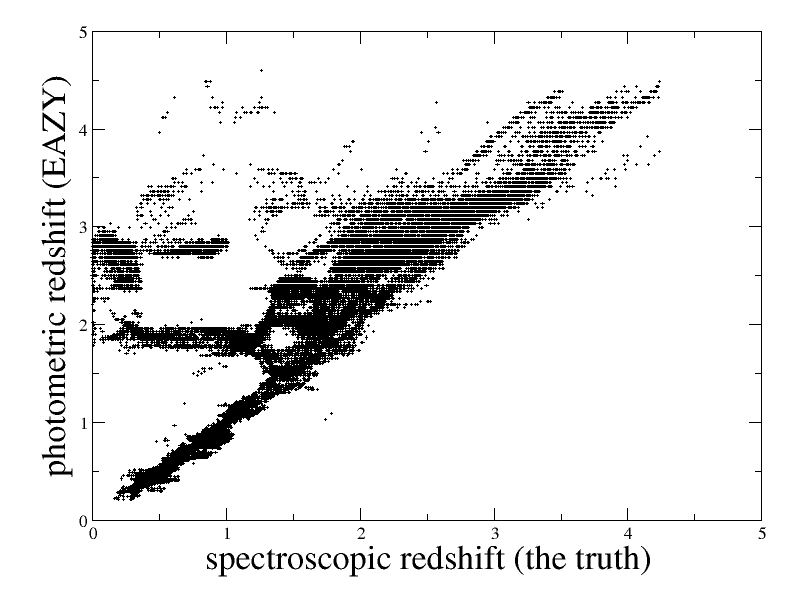
\includegraphics[scale=0.25]{eazy_scatter_plot.png}
\label{subfig:eazy}
}
\subfigure[]{
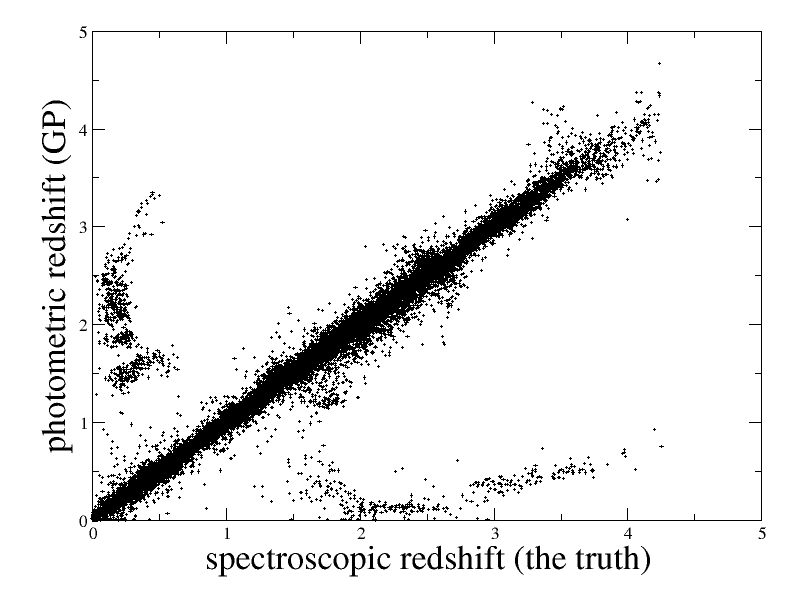
\includegraphics[scale=0.25]{gp_scatter_plot.png}
\label{subfig:gp}
}
\caption{
Photometric redshift plotted
against true spectroscopic redshift for 48,000 simulated LSST galaxy
observations.  Photometric redshifts are derived using the
EAZY template-fitting
algorithm (a forward model) in Figure \ref{subfig:eazy} and
our GP based algorithm in Figure \ref{subfig:gp}.
}
\label{fig:scatter}
\end{figure}

Other data-driven algorithms for photometric redshift determination do exist. 
An example of these is the publically-available code ANNz \cite{annz},
which is based on an artificial neural network scheme.
In this case, the principal
shortcoming  is that the artificial neural network
is designed to return only a
photometric redshift value and an uncertainty.
This uncertainty is a heuristic combination of the uncertainties in the
photometric data as well as the scatter in $z_\text{photometric}$ derived
from multiple instantiations of ANNz.  There is no guarantee that it represents
the true, probabilistic uncertainty in $z_\text{photometric}$.
Figure \ref{fig:lnsum} plots the mean value of $\ln[P(\text{truth})]$,
i.e. the value of the logarithm $P(z_\text{photometric})$ at the point
$z_\text{photometric}=z_\text{spectroscopic}$, 
as a function
of photometric redshift for EAZY, ANNz, and our GP algorithm.
We see that both EAZY and ANNz consistently assign lower probabilities to
$z_\text{photometric}=z_\text{spectroscopic}$ than does our GP algorithm.

Other works have attempted to apply GPs to the problem of
photometric redshfifts \cite{kaufman,bonfield}, however, they have treated
the problem as one of learning the form of a one-to-one scalar function.
We propose to use the probabilistic nature of GPs to learn the full
probability distribution that a given galaxy is at a given redshift.  The
resulting prediction is simultaneously more robust against sparse, noisy or
degenerate training data, more usable in follow-up scientific analyses, and
more amenable to model improvement by the introduction of active learning.
% Figure \ref{subfig:gp} shows preliminary results from our algorithm when
% trained on spectroscopic data from 50,000 galaxies and tested on the same
% 48,000 galaxies as Figure \ref{subfig:eazy}.  Here we see that the GP
% modeling yields significantly less scatter about the true
% $z_\text{photometric}=z_\text{spectroscopic}$ relationship.

\begin{figure}[t]
\centerline{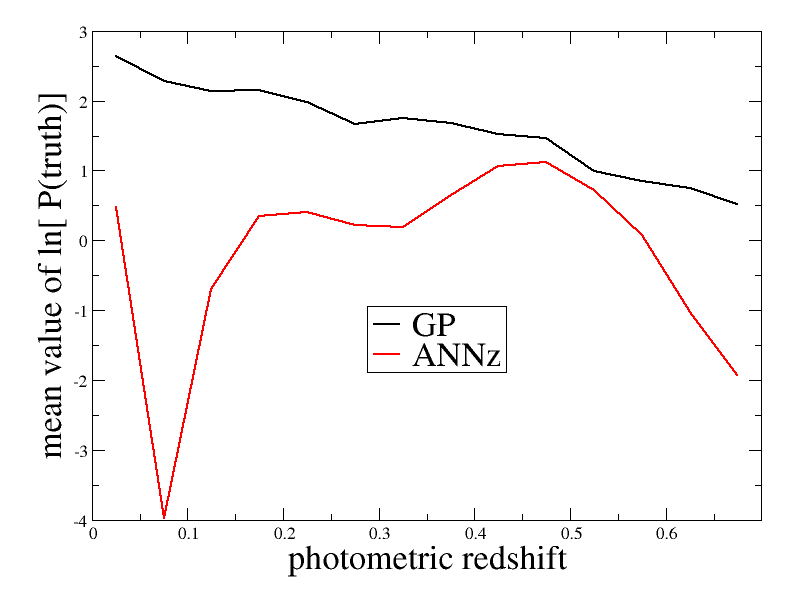
\includegraphics[scale=0.3]{sdss_lnsum.png}}
\caption{
The mean value of
$\ln[P(\text{truth})]$ as a function of photometric redshift (the vertical
axes in Figures \ref{fig:scatter}) for all
three algorithms under consideration using real
data taken from the Sloan Digital Sky Survey \cite{Abazajian:2008wr}.  
In this latter case, the
algorithms are trained on 21,000 galaxies and tested on 191,000 galaxies.
}
\label{fig:lnsum}
\end{figure}

The tests considered above represent idealized cases.
The algorithm resulting in Figure \ref{fig:scatter} was trained on high
signal-to-noise data with a training set sampled everywhere in
$z_\text{spectroscopic}$-space.  The algorithm resulting in Figure
\ref{fig:lnsum} is well-behaved in that the low redshift regime considered
exhibits no degeneracies in the photometry-to-redshift relationship.  This will
not be the case for the large, deep surveys of the future.  In order to extend
the favorable results of GPs above, further development of the
framework will be required.

\subsection{Fortifying Gaussian Processes against incomplete training data}
\label{sec:sparse}


GPs are already designed to handle input data that is sparsely
sampled.  Eqn \ref{eq:cov} gives the GP the freedom to declare a large
uncertainty in regions of data space where there is no training data.  However,
in order to deliver on the science results required by DES, LSST, and other
big-data surveys, it is not enough that $\Sigma_q$ be large where the model is
uncertain.  We require that the inferred 
value $f_q$ in Eqn \ref{eq:mean} be an accurate
representation of the true underlying model.  
We propose to achieve this in several ways.

\vspace{.5\baselineskip}
\begin{itemize}
\item New mean function models -- as presented,
Eqn \ref{eq:mean} sets the value of $\bar{y}$ to the algebraic mean of the
training outputs $\vec{y}$.  This assumes that the GP for all 
parameters $\vec{\theta}_q$
starts from the same value and Eqn \ref{eq:mean} expands the
departures from that value.  
We will evaluate models more complex than the algebraic
mean but simpler than the GP, which can be used to give a more informative value
for $\bar{y}$ such that it interpolates over gaps in the training data.  We propose
to experiment with functions including those using a basis
function representation of the function models. For example, a preliminary analysis using
 principal component
analysis on the input $\{\vec{\theta}\}$ to set $\bar{y}$ according to a linear
regression on the principal component most correlated 
with the outputs $\vec{y}$
shows an  improvement in the peformance of
the GP as a function regressor.

\item Dynamic hyper parameters -- the value of the characteristic
length scale $\ell$ in the covariance function $K_{ij}$ is presented
as a parameter to be optimized by cross-validation.  This, again, selects a
single value for $\ell$ for all possible $\vec{\theta}_q$, regardless of
$\vec{\theta}_q$'s position in the data space.  We will develop 
dynamic algorithms based on the covariance
structure present within the input $\{\vec{\theta}\,y\}$  
for setting $\ell$ so that highly-sampled 
training data will
return small $\ell$ (tightly coupling the GP to the training data) and
sparsely-sampled training data will give larger $\ell$, allowing for broader
interpolation across gaps in the training data.

\item Learned $K_{ij}$ -- in the above discussion, the functional form of
the covariance function
$K_{ij}$ in Eqn \ref{eq:covariogram}
was assumed.  
%While this certainly resulted in acceptable behavior in
%our test cases, 
It is, however, by no means guaranteed that the choice we made (a Gaussian
function in data space) will always be the best.  
We will explore ways
to enable the GP to learn the most appropriate form of 
the covariogram
based on the training data at hand. Examples of this include setting the
form of the covariance function
using cross-validation and information-theoretical
approaches that attempt to find a relationship between the form of the covariance
function and the entropy of the distribution produced by the GP.
\end{itemize}
\vspace{.5\baselineskip}

\subsection{Fortifying Gaussian Processes against degenerate training data}
\label{sec:multimode}

It will be necessary to build GPs that are robust against degeneracies
that exist in the relationship between input and output
data.  This pitfall can already be seen in the simulated photometric redshifts
plotted in Figure \ref{subfig:gp}.  Note the high
$z_\text{spectroscopic}$ galaxies that appear at low $z_\text{photometric}$ and
vice-versa.  To correct for this error, we will harness the full probabilistic
nature of GPs, building a system which tests the simplest, single-mode Gaussian
model against multi-modal models.  The proposed algorithm will work as
follows:
\vspace{.5\baselineskip}
\begin{enumerate}
\item Fit the training data to a single-mode GP.

\item Use Bayesian model selection \cite{mackay}
to compute the model likelihood of this single-mode GP.

\item Divide the training data into two sub-populations based on their output
values.

\item Fit each sub-population to its own GP.

\item Compute the model likelihood of this two-mode model and compare to the
model likelihood of the single-mode model.

\item Repeat steps 3-5 for three-mode, four-mode, etc. models until
  the system converges to the best fit to the training data.
\end{enumerate}

\vspace{.5\baselineskip}
Through this iterative approach, we expect to build  GPs such that, even when 
they
succumb to the degeneracies seen in Figure \ref{subfig:gp}, 
they will still place
significant probability density at the true
$z_\text{photometric}=z_\text{spectroscopic}$ value.  This will represent a
signtificant improvement over current model-learning algorithms, which are
principally concerned with returning a learned value for the model function and
some heuristic estimate for the uncertainty (i.e. neural networks).

\section{Active Learning}
\label{sec:active_learning}

A generic active learning algorithm takes the following form:

\vspace{.5\baselineskip}
\begin{enumerate}

\item Learn a model (e.g. a Gaussian process) using the current set of
  labeled training data.

\item Evaluate the set or space of unlabeled data according to some active
  learning criterion, usually beginning by requesting the predictive
  distribution from the learned model.

\item Choose the data point/experiment with the highest evaluation and
  obtain the label for it (e.g. by requesting a data collection experiment
  and/or asking a human expert to provide the label).

\item Add the resulting data to the training data and repeat.

\end{enumerate}
\vspace{.5\baselineskip}

The performance of an active learning algorithm is evaluated by some
measure of the model's quality (e.g. accuracy or log-likelihood on a test
set of data) as a function of the number of data points collected for the
training set.  The key algorithmic components are the model used in step 1
and the selection criterion used in step 2.  The previous section proposed
work on improving GP models.  In this section we propose new selection
criteria.

%We discuss specifically how we model $P(z_\text{photometric})$ below.

%Galaxy observations are represented as vectors $\{\vec{\theta}_q\}$ of
%flux information.  For each unknown
%test galaxy $\{\vec{\theta}_q\}$, we find the $k$ nearest neighbor training
%galaxies in flux space ($k$ is treated as a parameter to be optimized by our
%algorithm).  We divide these neighbor galaxies into two sub-populations based on
%their spectroscopic redshifts and fit a Gaussian Process to each sub-population.
%This gives us a bi-modal probability distribution for $P(z_\text{photometric})$. 
%We compare the likelihood of this hypothesis to a single-mode
%$P(z_\text{photometric})$ in which all of the neighbor galaxies are fit together
%in one Gaussian Process.  The final $P(z_\text{photometric})$ is a linear
%combination of these two hypotheses, weighted according to their respective
%model likelihoods.

\subsection{Novel active learning criteria}

\begin{figure}[t]
\centerline{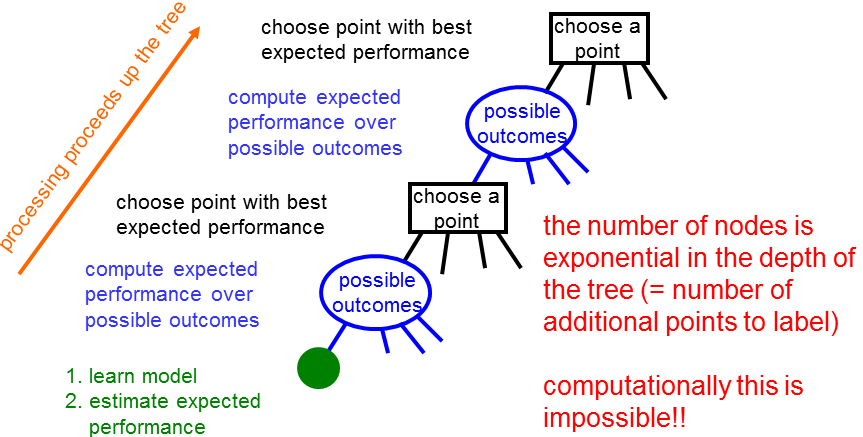
\includegraphics[scale=0.4]{searchtree.png}}
\caption{Search tree for an optimal active learning algorithm that will
  choose two more data points.}
\label{fig:searchtree}
\end{figure}

It is useful to see the challenges involved in developing good active
learning criteria by considering what an optimal algorithm might need to
do.  Figure \ref{fig:searchtree} shows the computation it would require.
The root of the tree contains the current decision on which point to choose
and an optimal algorithm would consider them all.  For each potential
choice, it would then consider every possible outcome (label) that might be
obtained and weight them by the estimated probability of each outcome.  For
each outcome, it would then consider what next point it would choose if it
received that outcome.  The tree expands down to a depth equal to the
number of data points that will be chosen and at the leaf every possible
model would be learned and evaluated.  The algorithm only chooses a new
point to label (the decision signified by the root of the tree) after it
has evaluated all possible choices out to their ultimate consequence.
Since the number of leaves is exponential in the depth of the tree, this
quickly becomes intractable.  A typical solution (referred to as myopic) is
to truncate the tree to zero or one level.  A second speedup is often
obtained by replacing a full model evaluation with a fast heuristic (see
reference \cite{Settles09} for a summary of common heuristics).  In our
work \cite{YifeiMa12} and others (e.g. \cite{Krause08}), myopic algorithms
can often be justified theoretically by using submodularity to show that
they obtain a performance within at least $1 - 1/e$ of optimal.

The evaluation of the model, whether in a full or truncated tree, is also a
challenge.  If we knew the true labels in our test set, we could use them
to evaluate the accuracy or log-likelihood of the true labels.  In a
simulated problem this is possible, but in a real application we do not
have the labels.  The usual alternative is to consider the uncertainty in
the predictions on the test points.  In the case of basic GPs, the
distribution is a multivariate Gaussian with covariance $\Sigma_q$ from
Eqn \ref{eq:cov} and the query is the entire test set.

A myopic information gain (change in entropy) strategy looks ahead one step
and chooses the data point that minimizes the expected entropy (monotonic
in $\det(\Sigma_q)$).  Even this can be expensive since it requires the
computation of the determinant.  An alternative is minimizing the average
variance $\text{tr}(\Sigma_q)$ (also known as V-optimality).  A further
approximation is to do no look ahead and simply choose the data point
corresponding to the largest diagonal element in $\text{tr}(\Sigma_q)$.  This is
known as uncertainty sampling.

We propose the following new methods:

\vspace{.5\baselineskip}
\begin{itemize}

\item The usual implementations of the criteria listed above are based on
  Gaussian predictive distributions which means only the covariance need be
  considered.  We will develop efficient ways to estimate these quantities
  from our improved models of non-Guassian distributions.  Two obvious criteria to try
  are the entropy of the output distribution or the logarithm of the probability
  distribution evaluated at its peak (which we use in the toy model
  generating Figure \ref{fig:learning}).

\item Our preliminary experiments on classification in graphs indicate that
  the sum of all entries in the covariance matrix is a better criterion
  than the trace \cite{YifeiMa12}.  We propose to develop an analogous
  criterion for euclidean spaces and for regression problems.  This
  criterion has not been previously proposed in the experiment design
  literature and we will also analyze theoretically when and why it
  outperforms the alternatives.

\item We can improve performance if we find the computational tricks needed
  to look ahead further.  Previously, we published a method for increasing
  look ahead in an active search problem by pruning the search tree
  \cite{Garnett12}.  It drastically reduces computation while provably
  returning the correct answer (i.e. not an approximation).  We propose to
  develop analogous pruning rules for the active learning problem.  We will
  further extend both methods by developing approximate pruning rules that
  trade off the aggressiveness of pruning, and thus the amount of look
  ahead allowed, against approximation accuracy.  We will investigate when
  the additional look ahead allowed more than compensates for the errors
  induced by aggressive pruning.

\end{itemize}
\vspace{.5\baselineskip}

% We will expand upon
% our recent work on the problem of optimal surveying or polling
% (Garnett et al 2012a).  Rather than having a goal of correctly
% predicting the output for each point in a test set, the goal is to
% predict the average output (or the class proportions in classification
% problems) over the test set.  This dramatically increases the
% efficiency of the active learning.  In preliminary experiments on
% graphs and other domains, minimizing this survey variance not only
% performs well on the surveying problem, but also outperforms the trace
% criterion and other popular active learning methods such as
% uncertainty and density sampling on active learning problems.
% This result is consistent with the findings of Richards {\it et al.} (2012b),
% who consider a similar problem for a Random Forest classifier on 
% the static data set produced by the All Sky Automated Survey.
% Intuitively, it seems reasonable that considering the entire
% covariance matrix of the modeled data
% might lead to better performance than choosing only
% based on its diagonal.  We have, however, little theoretical understanding of
% why this is better than the trace criterion which directly optimizes
% the quantity on which we will ultimately measure performance.  We will
% seek a better theoretical understanding of this phenomenon as part of
% this work.

\subsection{Active learning for photometric redshifts}

\begin{figure}[t]
\centerline{
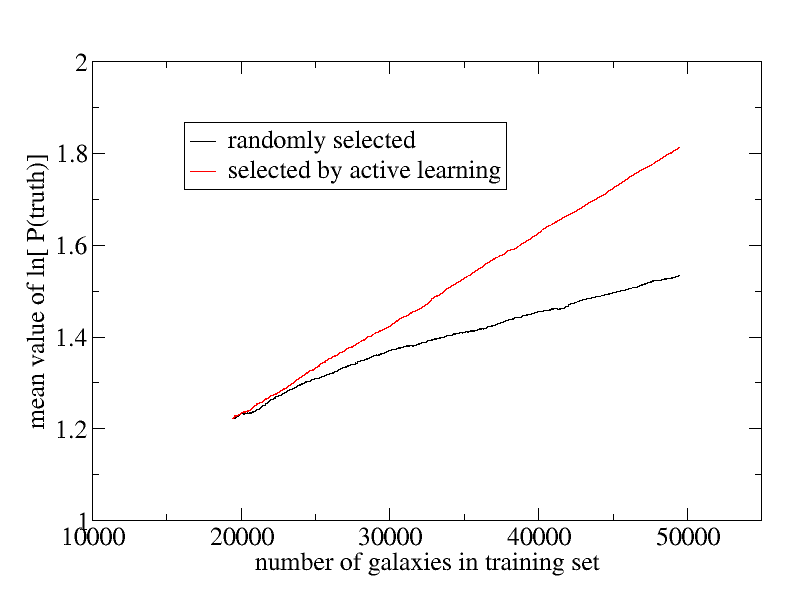
\includegraphics[scale=0.4]{learning_curve.png}
}
\caption{
Active learning applied to classification according to a scalar function on a
6-dimensional data space.  The horizontal axis is the size of the training data
set.  The vertical axis is the mean value of the output probability distribution
at the true value of the scalar function.  The black curve assembles the
training set randomly.  The red curve selects new training points that maximize
the figure of merit $\left(-\ln[P(\text{mode})]\right)$.
}
\label{fig:learning}
\end{figure}

In both empirical and forward-fitting photometric redshift codes, biases
arise from the fact that the distribution of training samples (templates)
is not the same in color and redshift space as the data the model will be
applied to.  Additional issues include the fact that some regions of color
space and some redshifts are more difficult to learn (require more training
samples).  We will show how our novel active learning algorithms can
achieve further improvements by choosing the most useful galaxies for
follow-up spectroscopy.

In a preliminary study we used a fully labeled data set containing galaxies
with both color measurements and true (spectroscopically determined)
redshift labels.  We simulated active learning by hiding the labels from
the GP learner and then providing them as requested by an active learning
algorithm.  We compared uniform random selection against uncertainty
sampling.  Figure \ref{fig:learning} demonstrates the results using the
problem presented in Figure \ref{fig:scatter}. %From a total of 97,000 data
%points, 
We start with 20,000 training points (consistent with the size of
current training sets used for photometric redshifts) and assess the efficacy of our
GP classifier by considering the mean value of $\ln[P(\text{truth})]$ as in
Figure \ref{fig:lnsum}.  Using this simplified active learning to add
to our training sample (as opposed to a random sampling strategy) 
leads to a significant improvement in the classifier's performance.

This study was done in a high signal-to-noise regime.  It takes no account
of the relative cost of doing one measurement or another.  No gaps exist in
the available training data.  These are all challenges that real-world
machine learning algorithms will face (see Section~\ref{sec:sparse}).
We will, therefore, develop our novel
methods on real data sets that contain all these additional challenges.

\begin{figure}[t]
\centerline{
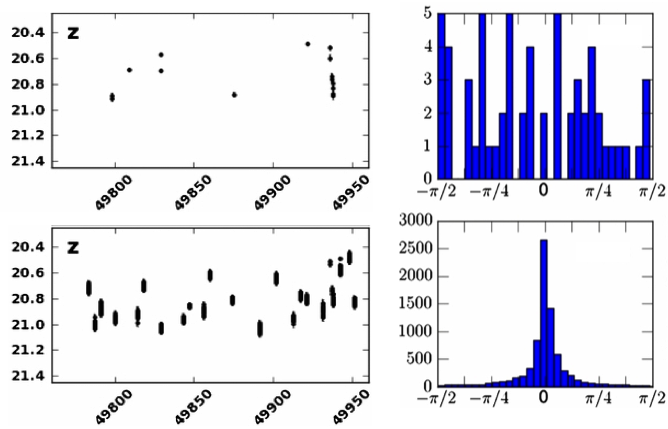
\includegraphics[scale=1.0]{rrlyrae.png}
}
\caption{
Taken from reference \cite{rrlyrae} the left panels shows the expected
sampling of
a light curve by the LSST at its main survey cadence (top left) and
for a higher sampling rate that will be employed for 10\% of the LSST
survey (bottom left). The right panels shows a measure of the  how well
the light curves can be characterized after phasing (i.e.\ after combining the observations while solving
for the periodicity of the data). Poorly sampled data are clearly
difficult to phase and classify. Active learning techniques can target
the next ``best'' observation enabling the improvements in
classification we see for highly sampled data but at the smallest observational cost.}

\label{fig:RRLyrae}
\end{figure}

\subsection{Active Learning for Classification}
\label{sec:transients}

Real-time automatic recognition and classification of transient objects and
events is already widely acknowledged as a necessary support technology for
the forthcoming age of survey cosmology
\cite{djorgovski2011,richards2011,richards2012,graham2012,mahabal2008a,mahabal2011a}.
The transient classification problem mirrors the photometric redshift
problem.  It is cheap and easy to get the initial observations of many
transients.  LSST will find thousands of them every night.  However,
obtaining an accurate ground-truth label of the object's type requires the
detection to be followed-up with other telescopes to measure the light
curves over time in multiple bands.  Getting a final label may also require
a human expert to analyze the light curves.  All of this is expensive.  As
with photometric redshifts, we propose to use our active learning
algorithms to choose which transients should be followed up.  

A great deal of work has already been accomplished developing algorithms
that can learn the classification of a transient object given data that are
well sampled and that are analysed in a batch mode. Even with these
idealized data sets misclassification rates are typically 30\% or greater.
For the DES and the LSST data streams these challenges are exacerbated as
the data are poorly sampled in the temporal domain and the classifications
must be undertaken in almost real-time (within 60s of an observation for
the case of the LSST).  For the case of the LSST 90\% of the data will be
sampled at a rate 20-times less than the highest cadence (with the highest
sampling rates undertaken in the ``Deep Drilling Fields'').
Figure~\ref{fig:RRLyrae} shows how this reduction in sampling degrades our
ability to constrain a light curve (and thereby classify a source).

We propose to break down the observations of a given object into $\{\Delta
m,\Delta t\}$ pairs (where $m$ is brightness and $t$ is time) as an input
to a GP regression and then classify the object based on that
reconstruction. Extension of the GP to return a probabilistic
reconstruction will enable active learning as well as the active feature
acquisition and active search algorithms described in the next section. For
lower signal-to-noise observations we propose to build the classification
model using basis functions derived from a decomposition of light curves
learned from the ``Deep Drilling Fields'' data (i.e.\ data with high
temporal sampling).

\subsection{The Challenge of Transients}

Transient objects present many additional challenges not addressed by a
basic active learning algorithm.  A decision to follow up is not done only
with the goal of improving the learned model.  The overarching science
dictates that some transients are of a more valuable type than others and
thus we want to maximize the number and quality of the light curves we
collect from them independently of any model learning considerations.  For
example, an object that doesn't fall into any existing class is especially
interesting while an object that turns out not to be a transient at all
(i.e. detected only because of noise) is scientifically worthless.  While
the latter might be valuable for improving our classifier, we ultimately
want to maximize the follow-ups done on the former.  This is called the
{\em active search problem}.

A second challenge is that follow up is not a single binary decision.
Choices must be made about what color bands to measure and at what timing
and frequency.  These choices might be revisited continously throughout the
follow up process.  This is called the {\em active feature acquisition
  problem}. Small errors in the identification and classification of transient
sources will swamp the system.  The LSST will detect 7.5x10$^8$ sources
{\bf every night}.  Even for the most numerous transient events (SNe), less
than 10$^{-5}$ of the total number of sources will belong to this class.
The most energetic bursters are 500 times rarer.  Algorithms for
identifying anomalies and variability must, therefore, be robust to false
positives and missing data and must account for the cadence in how we
sample the time domain, variations in the quality of the data due to
atmospheric conditions, changes in the performance of the telescope and
camera and the possibility that we observe sources at different wavelengths
at different times.

Finally, transient classification and active learning must be done in real
time.  Where a non-variable object's spectrographic redshift could be measured years
after its photometry was collected, a decision to follow up on a transient
must be taken in seconds or minutes. Otherwise, valuable data
might fade before it can be captured.  With timescales as short as seconds
to hours we require the ability to identify, classify and report any
detection in time to allow for follow-up observations before the initial
phenomenon fades.

All of these issues arise in the real-time data collection of any science
interested in the dynamics of a physical system.  Interestingly, the
problem is increasingly present in simulation efforts.  As simulations get
larger, it is impossible to store all the data and online decisions must be
made about what simulated variables and events merit the limited disk space
available.  While we focus our demonstration and testing on astrophysical
transients, our core algorithms will be generic enough to apply across
other scientific applications.

%The next generation of astrophysical surveys will visit the same
%region of sky many thousands of times. This opening of the temporal
%domain in astrophysics offers the potential to discover new classes of
%physical phenomena while coming with many associated computational
%challenges. Variability within the universe is believed to be present
%on time scales of seconds through to tens of years. The shortest time
%scales correspond to the explosion of the most massive stars within
%the universe which produce short but intense optical and gamma-ray
%flashes. These outbursts provide direct tests of General Relativity
%and of high energy physical processes (at energies far beyond those
%accessible on the Earth). For example the rate at which these events
%occur constrains the age at which the first stars within the universe
%came into being. Intermediate timescale variability comes in the form
%of supernovae (SNe) which detonate, brighten and then dim. These
%exploding stars are known to have a narrow range of intrinsic
%brightnesses; they act as standard candles that can be used to
%determine the rate at which the universe expands and thereby measure
%its mass and energy content \cite{perlmutter99}. 
%Longer time scale
%variablity (including variability due to the velocity of sources)
%comes from variations in the luminosity of acretion disks around black
%holes, the motion of stars throughout our Galaxy and the motion of
%asteroids within the local solar system. These...
%With surveys such as the LSST we will detect 250,000 SNe per year
%increasing the accuracy of measures of the energy content of the
%universe by an order of magnitude.
%

\section{Active Search}
\label{sec:active_search}

The active search problem and the Bayesian optimal algorithm for it are
described in our recent work \cite{Garnett11,Garnett12}.  An active search
algorithm proceeds exactly as the generic active learning algorithm give in
section \ref{sec:active_learning}.  Data is collected and the model is
improved.  The difference is the ultimate objective function.  Rather than
being evaluated on model quality with accuracy or log-likelihood, the goal
is to maximize the sum of the value of the objects selected for labeling.
For this discussion we simplify to a problem with only two classes: a
positive class worth one point and a negative class worth nothing.  A good
algorithm will still choose points that improve its model because the model
will help it find more positives in the future.  The tradeoff between
selecting known positives versus improving the model in the hopes of
finding more later is well known as the exploration/exploitation tradeoff.

As with active learning, an optimal algorithm would look like the search
tree in Figure~\ref{fig:searchtree}.  The difference is that the evaluation
in each leaf is the computation of the number of positives found.  A
computationally efficient active search method needs to find ways to cut
the search short and/or replace the computation of expensive expectations
with simple heuristics.  We propose the following new methods:
\vspace{.5\baselineskip}
\begin{itemize}
\item Approximate pruning rules in the spirit of the exact rules in reference
  \cite{Garnett12} that can trade off accuracy for search speed.

\item In reference \cite{Wang13} we showed how to combine an exact one-step myopic
  evaluation with an approximation of the future impact on positives found
  that could achieve results better than expensive look aheads on graph problems.
  We will develop analogous methods for Euclidean spaces and multi-class or
  real-valued outcomes, and will seek a theoretical characterization of the
  performance.

\item There is a large literature on bandit problems including the optimal
  algorithms derived from allocation indices when the alternatives are
  independent (see reference \cite{Gittin89}) and the more recent approaches based on
  obtaining provable regret bounds (see reference \cite{Auer02} and the extensive
  work after it).  Bandit problems are about finding good choices and
  exploiting them repeatedly.  Active search is different because each
  selection pays off at most once and the key is using that information to
  quickly find other valuable selections.  Nonetheless, there are
  similarities and we will investigate when and how bandit algorithms can
  be adapted to do active search.

\end{itemize}
\vspace{.5\baselineskip}

\section{Active Feature Acquisition}

In the work discussed so far, we have considered the process of acquiring a
label to be a single decision to do so.  The active learning or search
algorithm looks at the feature data, and then decides whether to request
the label.  If it does, the label is obtained through a single expensive
experiment.  Here we consider the case where many possible features can be
measured and each increases the accuracy of the label prediction.

We propose to build active feature acquisition methods on a Gaussian
process based classifier where a GP is created for each class with
different priors according to the class.  When data from a new object
arrives, it is applied to the GP for each class and the posterior class
probability is computed by applying Bayes rule to the likelihood of each
model.  This GP model follows the approach we used recently to detect
damped lyman alpha (DLA) systems in the spectra of quasars
\cite{Garnett12a}.

Using the GP equations from section \ref{sec:gp} on the model for each
class, we can get a mean and covariance for any set of unobserved features
under the assumption that class is the correct one.  We then use the
posterior class probabilities to get a combined distribution over what we
expect to see if we choose to observe some currently unobserved feature.
The result is a set of joint prediction distributions over all class labels
and unobserved features.  These distributions are what we need to
instantiate an information theoretic version of figure \ref{fig:searchtree}
for the active feature acquisition problem.  The nodes that consider all
possible outcomes become integrals over the combined distribution of
expected observations.  The evaluation function in the leaves is the
entropy of posterior class probabilities: $H(X) = -\Sigma_k p_k \log(p_k)$
where $p_k$ is the posterior probability that discrete random variable $X$
has value $k$.  As with active learning and active search, we will use a
truncated search tree in order to obtain a tractable myopic algorithm.

\subsection{Application to transients}

A GP for the transient classification problem will have two dimensions, one
for time and the other for color band or wavelength.  The active feature
acquisition problem will have additional constraints because the
opportunity to observe features will proceed along the time dimension and
an instantaneous decision to observe that time-color combination or pass it
up forever will have to be made.  The search tree can be modified
accordingly by restricting the observations available at each ``choose
node''.

The good performance of myopic algorithms, both practically and
theoretically, depends on a diminishing returns property that assumes an
observation you skipped at one time point can always be made at a later
time.  This obviously is not possible with transients.  When deciding on an
observation, not only its current information content is important.  You
must also consider whether observations you might take in the future might
be a good proxy for the one currently under consideration.  To overcome
this issue, we propose a calibration scheme that reviews previously
observed objects and learns an adaptive threshold on the myopic information
gain that can be applied to new objects.

% \subsection{Group-based Active Feature Acquisition and Active Search
% for Transient Classification}
% 
% The active learning, active search, and active feature
% acquisition choices for transient classification
% all must be made in an online, streaming fashion.  
% Rather than
% considering an entire pool of test objects, they appear one at a time as
% they are detected and the algorithm must decide whether and how to follow
% up on each immediately as they are detected. 
% The input features for transient object classification will be 
% a variable combination photometric
% and morphologic measures taken at different increments in time. With
% this proposal we will  introduce an information-theoretical approach 
% based on the output covariance matrix of Eqn \ref{eq:cov} which will allow
% us to perform a similar determination in real time as observations are made,
% directing experiments as they are performed.
% We will not choose our follow-up observations based on cross-validation testing,
% but rather based on which observations we expect to yield the most significant
% decreases in the entropy of our probabilistic model.
% References \cite{huijse2011,huijse2012} use a similar scheme to find the correlation
% between observations within a single light curve.  We will attempt to find
% the type of observation with the greatest information content. 

\section{Integration and Computation}

The culmination of our proposed program of research will be to integrate
the methods devised above into a single, combined, computationally
efficient streaming algorithm.  The three goals of active learning, active
search, and active feature acquisition will be combined in a staged set of
decisions.  When a new event or object is detected, the data will be used
to provide an estimated physical model for the object.  These models are
the input variables for this object in the active learning and active
search algorithms.  In parallel, the active learning and active search
methods will decide whether to follow-up on this object.  If either of them
selects the object, it is advanced to active feature acquisition.  There
additional observations on the object are selected and the process for this
object repeats.  An object that initially seemed interesting to one
algorithm may cease to be so after additional observations or may be
adopted by the other one.  The process for one object terminates when
neither active learning nor active search remains interested in it or the
object class and light curves are characterized well enough that no more
observations are required.

% Finally, we propose to expand on these approaches to operate on groups of
% objects
% statistics to consider not just individual anomalies but also group
% anomaly detection algorithms that consider arbitrary groupings of
% self-similar anomalous records \cite{Neill05}.

\subsection{Caching structures for computational efficiency}
\label{sec:computationalefficiency}

Scaling our algorithms up to the size of future scientific data sets will
require a number of algorithmic, caching, statistical, and parallel
computation tricks.  We will draw from the following methods and ideas:

%\vspace{-4mm}
\paragraph{AD-Trees.}
The AD-Tree \cite{Moore97a} caching structure has the feature that it can
answer any count query (i.e. how many records match query X?) in time
independent of the number of records.  It is similar to an OLAP datacube,
except that it caches the answer to all possible queries in a single
structure rather than requiring the building of many cubes.  Specialized
pruning tricks keep its memory footprint modest.  Our algorithms will rely
heavily on this structure. A structure called a TCube extends AD-Trees to
time series \cite{Sabhnani06}.  This allows queries of the form: {\it
  return the aggregated time series of counts for all records matching
  query X}.  Additional pruning tricks based on sparse vector
representations allow this to be memory efficient.

We propose additional modifications that will cache sufficient statistics.
In addition to counts, it will store means and covariances of
continuous-valued attributes.  This is especially useful for search-based
comparison techniques because those sufficient statistics can be used to
build classifiers such as LDA or QDA, which can quickly assess whether
there is a difference between two populations of objects.
%  This allows an efficient rule-based
%search for sub-populations with differences between them in the same way it
% was done in the Radsearch algorithm \cite{Moore02}.

%\vspace{-4mm}
\paragraph{KD-Trees.}
KD-Trees are classic data structures used extensively in machine learning
and N-body simulations.  A traditional use is to retrieve nearest neighbors
in {\it log N} time.  By storing sufficient statistics at the internal
nodes of the trees, one can retrieve the statistics needed for operations
such as kernel regression very efficiently \cite{Moore97}.  KD-Trees are
especially valuable with GPs because a full GP requires a matrix inversion
of the size of the number of data points in the data set, which may be
intractable.  The typical GP kernel, however, has a locality property that
means the number of points contributing to any particular query is modest.  We will use KD-Trees to find these points efficiently.
% These also take {\it log N} time in all but pathological cases.  

%\vspace{-4mm}
\paragraph{Hierarchical search structures.}  
The field of scan statistics \cite{Kulldorf97,Neill03} has developed a set
of hierarchical structures specially designed for spatial-temporal data.
We will extend these for use in identifying interesting space-varying and
time-varying phenomenon.  The key feature is that when searching for
spatio-temporal anomalies or matches to patterns, the right choice of
scoring metric makes it possible to significantly prune the search space
(i.e. based on the sufficient statistics for this region, I can determine
that no sub-region will fit my criteria).

\paragraph{Distributed computation.}
The algorithms we propose may be further sped up by parallelizing across
CPUs on a grid.  We will use this technique when possible using standard
cloud computing paradigms \cite{gard07} and expect our efforts on efficient
algorithms, caching, and parallelization to yield speedups that compound on
each other.

\section{Timeline, Development Plan, and Responsibilities}

We will focus on multiple projects in each of the three years of this
program.  Algorithms will be released as they are developed in a
twice-yearly release cycle.  Algorithm development will be undertaken using
data from the DES survey, and a series of detailed simulations developed
for the LSST \cite{connolly10}.  Each item below will indicate which of the
PIs will take the lead in that stage of the program.

\noindent {\bf Year 1:}
\vspace{.5\baselineskip}
\begin{itemize}

\item (Schneider) Develop GP algorithms that are robust against sparse
  training data and capable of modeling multi-modal probability
  distributions.

\item (Connolly) Build a photometric redshift algorithm based on these new
  GPs.  Test the algorithm against data from the DES, and simulated LSST.

\item (Schneider) Develop active learning methods optimized for our new
  GPs.  Initially develop myopic criteria and later develop methods to
  increase look ahead.

\item (Connolly) Test the developed active learning methods on photometric
  redshift data.

\item (Schneider) Develop a software package for release to other scientists.

\end{itemize}
\vspace{.5\baselineskip}

\noindent {\bf Year 2:} 
\vspace{.5\baselineskip}
\begin{itemize}

\item (Schneider) Develop active feature acquisition algorithms.  Use them
  to determine what additional information (e.g., morphological or angular
  correlation function) provides the most helpful supplement information in
  the case of photometric redshifts.

\item (Connolly) Extend our GPs to the problem of transient-classification.
  Analyze stellar sources where there are known populations with defined
  variability signatures (e.g.\ Cepheid variables) to provide validation
  for the analysis.

\item (Connolly) Extend the active feature acquisition algorithms developed
  for photometric redshifts to the problem of determining the next best
  measurement for transient classification.  Validate these algorithms on
  DES, and simulated LSST observations.

\item (Schneider) Generalize our active learning and active feature
  acquisition algorithms beyond GPs to work with any probabilistic
  model-fitting algorithm.  Develop a software package providing access to
  these algorithms.

\end{itemize}
\vspace{.5\baselineskip}

\noindent {\bf Year 3:} \vspace{.5\baselineskip}

\begin{itemize}

\item (Schneider) Develop active search algorithms based on GPs and
  extended to other probabilistic models.

\item (Connolly) Integrate our active learning and active feature
  acquisition algorithms to produce an active search algorithm that can
  identify interesting objects and optimize their follow-up in real time
  data streams.  Begin running this algorithm on DES data as it is made
  public.

\item (Connolly,Schneider) Develop an integrated software package that will
  provide access to all of our algorithms for use by scientists across all
  fields.


\end{itemize}

\newpage


\section*{References}
\begin{thebibliography}{99}
\bibitem{Garnett11}

Garnett,~R., Krishnamurhty,~Y., Wang,~D., Schneider,~J., and Mann,~R. 2011,

``Bayesian Optimal Active Search on Graphs,'' KDD Workshop on Mining and

Learning with Graphs



\bibitem{Garnett12}

Garnett,~R., Krishnamurthy,~Y., Xiong,~X., Schneider,~J., and Mann,~R. 2012,

``Bayesian Optimal Active Search and Surveying,'' International Conference on

Machine Learning



\bibitem{straf03}

Straf,~M.~L. 2003, Journal of the American Statistical Association {\bf 98}, 1



\bibitem{GrayMoore}

Gray, A. G., Moore, A. W., Nichol, R. C., Connolly, A. J.,

Genovese, C., and Wasserman, L. 2004, Astronomical Society of the Pacific Conference

Proceedings {\bf 314} 249



\bibitem{kubica}

Kubica, J., Denneau, L., Jr., Moore, A., Jedicke, R., Connolly, A. 2007,

Astronomical Society of the Pacific Conference Series {\bf 376} 395



\bibitem{Scranton2002}

Scranton,~R., Johnston,~D., Dodelson,~S., Frieman,~J.~A., Connolly,~A.,

Eisenstein,~D.~J., Gunn,~J.~E., Hui,~L., Jain,~B., Kent,~S., Loveday,~J.,

Narayanan,~V., Nichol,~R.~C., O'Connell,~L., Soccimarro,~R., Sheth,~R.~K.,

Stebbins,~A., Strauss,~M.~A., Szalay,~A.~S., Sapudi,~I., Tegmark,~M.,

Vogeley,~M., Zehavi,~I., Annis,~J., Bahcall,~N.~A., Brinkman,~J., Csabai,~I.,

Hindsley,~R., Ivezic,~Z., Kim,~R.~S.~J., Knapp,~G.~R., Lamb,~D.~Q., Lee,~B.~C.,

Lupton,~R.~H., McKay,~T., Munn,~J., Peoples,~J., Pier,~J., Richards,~G.~T.,

Rockosi,~C., Schlegel,~D., Schneider,~D.~P., Stoughton,~C., Tucker,~D.~L.,

Yanny,~B., York,~D.~G. 2002, The Astrophysical Journal {\bf 579}, 48



\bibitem{Szapudi2002}

Szapud,~I., Frieman,~J.~A., Scoccimarro,~R., Szalay,~A.~S., Connolly,~A.~J.,

Dodelson,~S., Eisenstein,~D.~J., Gunn,~J.~E., Johnston,~D., Kent,~S.,

Loveday,~J., Meiksin,~A., Nichol,~R.~C., Scranton,~R., Stebbins,~A.,

Vogeley,~M.~S., Annis,~J., Bahcall,~N.~A., Brinkman,~J., Csabai,~I., Doi,~M.,

Fukigita,~M., Ivezi\'c,~\u Z., Kim,~R.~S.~J., Knapp,~G.~R., Lamb,~D.~Q.,

Lee,~B.~C., Lupton,~R.~H., McKay,~T.~A., Munn,~J., Peoples,~J., Pier,~J.,

Rockosi,~C., Schlegel,~D., Stoughtfon,~C., Tucker,~D.~L., Yanny,~B., York,~D.~G.

2002, The Astrophysical Journal {\bf 570}, 75



\bibitem{Nichol2006}

Nichol,~R.~C., Sheth,~R.~K., Suto,~Y., Gray,~A.~J., Kayo,~I., Wechsler,~R.~H.,

Marin,~F., Kulkarni,~G., Blanton,~M., Connolly,~A.~J., Gardner,~J.~P., Jain,~B.,

Miller,~C.~J., Moore,~A.~W., Pope,~A., Pun,~J., Schneider,~D., Schneider,~J.,

Szalay,~A., Szapudi,~I., Zehavi,~I., Bahcall,~N.~A., Csabai,~I., Brinkmann,~J.

2006, Monthly Notices of the Royal Astronomical Society {\bf 368}, 1507



\bibitem{mcbride2011a}

McBride,~C.~K., Connolly,~A.~J., Gardner,~J.~P., Scranton,~R., Newman,~J.~A.,

Scoccimarro,~R., Zehavi,~I., and Schneider,~D.~P. 2011, The Astrophysical

Journal, {\bf 726}, 13



\bibitem{mcbride2011b}

McBride,~C.~K., Connolly,~A.~J., Gardner,~J.~P., Scranton,~R., Scoccimarro,~R.,

Berlind,~A.~A., Mar\'in,~F., and Schneider,~D.~P. 2011, The Astrophysical

Journal {\bf 739}, 85



\bibitem{Skibba2006}

Skibba,~R., Sheth,~R.~K., Connolly,~A.~J., and Scranton,~R. 2006,

Monthly Notices of the Royal Astronomical Society, {\bf 369}, 68



\bibitem{yip2004a}

Yip,~C.~W., Connolly,~A.~J., Szalay,~A.~S., Budav\'ari,~T., SubbaRao,~M.,

Frieman,~J.~A., Nichol,~R.~C., Hopkins,~A.~M., York,~D.~G., Okamura,~S.,

Brinkmann,~J., Csabai,~I., Thakar,~A.~R., Fukugita,~M., 

and Ivezi\'c,~\u Z. 2004, The Astronomical Journal {\bf 128}, 585



\bibitem{vdp2009}

Vanderplas,~J. and Connolly,~A.~J. 2009,

Astronomical Journal {\bf 138}, 1365



%\cite{Daniel:2011rr}

\bibitem{daniel2011} 

  Daniel,~S.~F., Connolly,~A.~J., Schneider,~J., Vanderplas,~J. and Xiong,~L.

  2011, 

  %``Classification of Stellar Spectra with LLE,''

  The Astronomical Journal  {\bf 142}, 203

  [arXiv:1110.4646 [astro-ph.SR]].

  %%CITATION = ARXIV:1110.4646;%%



\bibitem{daniel2012}

Daniel,~S.~F., Connolly,~A.~J., and Schneider,~J. 2012

[arXiv:1205.2708]



\bibitem{YiZhangICML2010}

Zhang,~Y. and Schneider,~J. 2010, ``Projection Penalties: Dimension Reduction without

Loss,'' International Conference on Machine Learning



\bibitem{YiZhangSDM2010}

Zhang,~Y., Schneider,~J., and Dubrawski,~A. 2010,

``Learning Compressible Models,'' Proceedings of SIAM Data Mining Conference





\bibitem{YiZhangMultitask2010}

Zhang,~Y. and Schneider,~J. 2010,

``Learning Multiple Tasks with a Sparse Matrix-Normal Penalty,''

Neural Information Processing Systems





\bibitem{YiZhang2011multiECOC}

Zhang,~Y. and Schneider,~J 2011, ``Multi-label Output Codes using Canonical Correlation

Analysis,'' Artificial Intelligence and Statistics



\bibitem{YiZhang2012}

Zhang,~Y. and Schneider,~J. 2012, ``Maximum Margin Output Coding,''

International Conference on Machine Learning



\bibitem{poczos11alphadiv}

Poczos,~B. and Schneider,~J. 2011, ``On the Estimation of alpha-Divergences,''

Artificial Intelligence and Statistics (AISTATS)



\bibitem{Poczos2011UAI}

Poczos,~B., Xiong,~L., and Schneider,~J. 2011, ``Nonparametric Divergence Estimation with

Applications to Machine Learning on Distributions,''  Uncertainty in Artificial

Intelligence



\bibitem{poczos12CVPR}

Poczos,~B., Xiong,~L., Sutherland,~D., and Schneider,~J. 2012,

``Nonparametric Kernel Estimators for Image Classification,''

IEEE Conference on Computer Vision and Pattern Recognition



\bibitem{Xiong2011gad}

Xiong,~L., Poczos,~B., Schneider,~J., Connolly,~A., Vanderplas,~J. 2011,

``Hierarchical Probabilistic Models for Group Anomaly Detection,''

Artificial Intelligence and Statistics (AISTATS)



\bibitem{xiong2011fgm}

Xiong,~L., Poczos,~B., and Schneider,~J. 2011, ``Group Anomaly Detection using Flexible

Genre Models,'' Neural Information Processing Systems



\bibitem{Tesch13}

Tesch, M., Schneider, J., and Choset, H. 2013,

``Expensive Funciton Optimization with Stochastic Binary Outcomes,''

in ``International Conference on Machine Learning (ICML)''



\bibitem{Wang13}

Wang, X., Garnett, R., and Schneider, J. 2013,

``Active Search on Graphs,'' in ``ACM SIGKDD Conference on Knowledge Discovery

and Data Mining''



\bibitem{Sutherland13}

Sutherland, D., Poczos, B. and Schneider, J. 2013,

``Active Learning and Search on Low-Rank Matrices,'' in

``ACM SIGKDD Conference on Knowledge Discovery and Data Mining''



\bibitem{kitching}

Kitching,~T.~D., Taylor,~A.~N., and Heavens,~A.~F. 2008,

Monthly Notices of the Royal Astronomical Society {\bf 389} 173



\bibitem{huterer2006}

Huterer,~D., Takada,~M., Bernstein,~G., and Jain,~B. 2006,

Monthly Notices of the Royal Astronomical Society {\bf 366}, 101



\bibitem{nakajima2011}

Nakajima,~R., Mandelbaum,~R., Seljak,~U., Cohn,~J.~D., Reyes,~R., and

Cool,~R. 2012, Monthly Notices of the Royal Astronomical Society {\bf 420}, 3240

[arXiv:1107.1395]



\bibitem{annz}

Collister,~A.~A. and Lahav,~O. 2004,

Publications of the Astronomical Society of the Pacific {\bf 116}, 345



\bibitem{gp}

Rasmussen, C.~E. and Williams, C.~K.~I., 2006, ``Gaussian

Processes for Machine Learning''

\verb|http://www.GaussianProcess.org/gpml/|



\bibitem{ericgp}

Shafieloo,~A., Kim,~A.~G., and Linder,~E.~V. 2012,

Physical Review D {\bf 85}, 123530 [arXiv:1204.2272]



\bibitem{psf}

Berg\'e,~J., Price,~S., Amara,~A., and Rhodes,~J. 2012,

Monthly Notices of the Royal Astronomical Society {\bf 419}, 2356



\bibitem{mahabal2008b}

Mahabal,~A., Djorgovski,~S.~G., Williams,~R., Drake,~A., Donalek,~C.,

Graham,~M., Moghaddam,~B., Turmon,~M., Jewell,~J., Khosla,~A., and

Hensley,~B. 2008 [arXiv:0810.4527] to appear in proceedings of the Class 2008

conference (Classification and Discovery in Large Astronomical Surveys, Ringberg

Castle, 14-17 October 2008)



\bibitem{wang2011}

Wang, Yuyang, Khardon, Roni, and Protopapas, Pavlos 2011

arXiv:1111.1315



\bibitem{wang2012}

Wang, Yuyang, Khardon, Roni, and Protopapas, Pavlos 2012

arXiv:1203.0970



\bibitem{huijse2011}

Huijse, Pablo, Est\'evez, Pablo A., Zegers, Pablo, Pr\'incipe, Jose C.,

and Protopapas, Pavlos 2011, IEEE Signal Processing Letters {\bf 18}, 371



\bibitem{huijse2012}

Huijse, Pablo, Est\'evez, Pablo A., Protopapas, Pavlos, Zebers, Pablo,

and Pr\'incipe, Jos\'e C. 2012, arXiv:1212.2398



\bibitem{Garnett12a}

Garnett,~R., Ho,~S., and Schneider,~J. 2012,

``Gaussian Processes for Identifying Damped Lyman-alpha Systems in Spectroscopic

Surveys,'' Neural Information Processing Systems 

workshop on Modern Nonparametric Methods in Machine Learning



\bibitem{Tesch11a}

Tesch, M., Schneider, J., and Choset, H. 2011,

``Adapting Control Policies for Expensive Systems to Changing Environments,'' in

``IEEE/RSJ International Conference on Intelligent Robots and Systems (IROS)''



\bibitem{Tesch11b}

Tesch, M., Schneider, J., and Choset, H. 2011,

``Using Response Surfaces and Expected Improvements to Optimize 

Snake Robot Gait Parameters,''

in

``IEEE/RSJ International Conference on Intelligent Robots and Systems (IROS)''





\bibitem{connolly95}

Connolly, A. J., Csabai, I., Szalay, A. S., Koo, D. C., Kron, R. G.,

and Munn, J. A. 1995, Astronomical Journal {\bf 110} 2655



\bibitem{eazy}

Brammer,~G.~B., van Dokkum,~P.~G., and Coppi,~P. 2008,

The Astrophysical Journal {\bf 686}, 1503





\bibitem{budavari2008}

Budav\'ari,~T. 2008 The Astrophysical Journal {\bf 695}, 747



\bibitem{kaufman}

Kaufman, Cari G., Bingham, Derek, Habib, Salman, Heitmann, Katrin, and Frieman,

Joshua A. 2011, The Annals of Applied Statistitcs {\bf 5} 2470



\bibitem{bonfield}

Bonfield,~D.~G., Sun,~Y., Davey,~N., Jarvis,~M.~J., Abdalla,~F.~B.,

Banerji,~M., Adams,~R.~G. 2010, Monthly Notices of the Royal Astronomical Society 

{\bf 405} 987



\bibitem{Abazajian:2008wr}

  Abazajian, K.~N.{\it et al.}  [SDSS Collaboration]~2009,

  %``The Seventh Data Release of the Sloan Digital Sky Survey,''

  The Astrophysical Journal Supplement Series  {\bf 182}, 543

  [arXiv:0812.0649 [astro-ph]].

  %%CITATION = APJSA,182,543;%%



\bibitem{mackay}

MacKay, David 1992, Neural Computation {\bf 4} 415



\bibitem{Settles09}

Settles,~B. 2009, ``Active Learning Literature Survey,'' Computer Sciences Technical

Report 1648, University of Wisconsin-Madison,

\verb|http://pages.cs.wisc.edu/~bsettles/active-learning/|



\bibitem{YifeiMa12}

Ma,~Y., Garnett,~R., and Schneider,~J. 2012,

``Submodularity in Batch Active Learning and Survey Problems

on Gaussian Random Fields,''

Neural Information Processing Systems 

workshop on Discrete Optimization in Machine Learning



\bibitem{Krause08}
A. Krause and A. Singh and C. Guestrin, 2008, 
``Near-optimal sensor placements in Gaussian processes: Theory,
efficient algorithms and empirical studies",
Journal of Machine Learning Research
\bibitem{rrlyrae}

Oluseyi, Hakeem M., Becker, Andrew C., Culliton, Christopher, Furqan, Muhammad,

Hoadley, Keri L., Regencia, Paul, Wells, Akeem J., Ivez\`ic, Zeljko, Jones, R.

Lynne, Krughoff, K. Simon, and Sesar, Branimir (2012), The Astronomical Joural

{\bf 144} 9





\bibitem{djorgovski2011}

Djorgovski,~S.~J., Donalek,~C., Mahabal,~A.~A., Moghaddam,~B., Turmon,~M.,

Graham,~M.~J., Drake,~A.~J., Sharma,~N. and Chen,~Y. 2011

[arXiv:1110.4655] to appear in Statistical Analysis and Data Mining, ref. proc.

CIDU 2011 conf., eds. A. Srivastava and N. Chawla



\bibitem{richards2011}

Richards,~J.~W., Starr,~D.~L., Butler,~N.~R., Bloom,~J.~S., Brewer,~J.~M.,

Crellin-Quick,~A., Higgins,~J., Kennedy,~R., and Rischard,~M. 2011,

The Astrophysical Journal {\bf 733}, 10



\bibitem{richards2012}

Richards,~J.~W., Starr,~D.~L., Brink,~H., Miller,~A.~A., Bloom,~J.~S.,

Butler,~N.~R., James,~J.~B., Long,~J.~P., and Rice,~J. 2012

The Astrophysical Journal {\bf 744}, 192



\bibitem{graham2012}

Graham,~M.~J., Djorgovski,~S.~G., Mahabal,~A., Donalek,~C., Drake,~A.,

Longo,~G. 2012 [arXiv:1208.2480] to appear in special issue of Distributed and

Parallel Databases on Data Intensive eScience



\bibitem{mahabal2008a}

Mahabal,~A., Djorgovski,~S.~G., Turmon,~M., Jewell,~J., Williams,~R.~R.,

Drake,~A.~J., Graham,~M.~G., Donalek,~C., Glikman,~E., and the Palomar-QUEST Team

2008, Astronomische Nachrichten {\bf 329}, 288





\bibitem{mahabal2011a}

Mahabal,~A.~A., Donalek,~C., Djorgovski,~S.~J., Drake,~A.~J.,

Graham,~M.~J., Williams,~R., Chen,~Y., Moghaddam,~B., and Turmon,~M.

2011, [arxiv:1111.3699] to appear in Proc. IAU 285, ``New Horizons in Transient

Astronomy,'' Oxford, September 2011



\bibitem{Gittin89}

Gittins, J. 1989, ``Multi-Armed Bandit Allocation Indices,'' published by Wiley



\bibitem{Auer02}

Auer, P., Cesa-Bianchi, N., and Fischer, P. 2002,

``Finite-time Analysis of the Multiarmed Bandit Probem,''

Machine Learning {\bf 47} 235



\bibitem{Neill05}

Neill, D. and Moore, A. 2005,

``Detecting Significant Multidimensional Spatial Clusters,''

Advances in Neural Information Processing Systems {\bf 17} 969



\bibitem{bryan}

Bryan, B., Schneider, J., Miller, C.~J., Nichol, R.~C., Genovese, C., and

Wasserman, L., 2007,

The Astrophysical Journal {\bf 665}, 25



\bibitem{kim2011}

Kim, Dae-Won, Protopapas, Pavlos, Byun, Young-Ik, Alcock, Charles, Khardon,

Roni, and Trichas, Markos 2011, arXiv:1101.3316



\bibitem{pichara2012}

Pichara, K., Protopapas, P., Kim, D.-W., Marquette, J.-B., and Tisserand, P.

2012, Monthly Notices of the Royal Astronomical Society, {\bf 427} 1284



\bibitem{brink2012}

Brink, Henrik, Richards, Joseph W., Poznanski, Dovi, Bloom, Joshua S., Rice,

John, Negahban, Sahand, and Wainwright, Martin 2012, arXiv:1209.3775



\bibitem{Moore97a}

Moore, A., and Lee, M. 1998, Journal of Artificial Intelligence Research {\bf 8} 67



\bibitem{Sabhnani06}

Sabhnani, M., Moore, A., and Dubrawski, A. 2006,

``T-Cube: A Data Structure for Fast Extraction of Time Series from Large Datasets,''

technical report number CMU-ML-06-104



\bibitem{Moore02}

Moore, A. W., and Schneider, J. G. 2002, 

``RADSEARCH: A new approach for finding optimal rules

efficiently from dense datasets,'' in ``AAAI-2002''



\bibitem{Moore97}

Moore, A., Schneider, J., and Deng, K. 1997,

``Efficient Locally Weighted Polynomial Regression Predictions,'' in

``International Conference on Machine Learning''



\bibitem{Moore99}

Moore, A. 1999, ``Very Fast EM-based Mixture Model Clustering using Multiresolution

Kd-trees,'' in ``Neural Information Processing Systems 11''  pp. 543-549



\bibitem{Kulldorf97}

Kulldorrff, M. 1997,

Communications in Statistics -- Theory and Methods {\bf 26} 1481





\bibitem{Neill03}

Neill, D. and Moore, A. 2003,

``A fast multi-resolution method for detection of significant spatial overdensities,''

Carnegie Mellon University Computer Science Department paper 2175





\bibitem{gard07}

Gardner, J. P., Connolly, A. J., and McBride, C. 2007,

``Enabling rapid development of parallel tree search applications,''

in ``Proceedings of the 2007 Workshop on Challenges of Large Applications in Distributed

Environments (CLADE)''



\bibitem{connolly10}

Connolly, A. J., Peterson, J., Jernigan, J. Garrett, Abel, Robert, Bankert, Justin,

Chang, Chihway, Claver, Charles F., Gibson, Robert, Gilmore, David K., Grace, Emily,

Johnes, R. Lynne, Ivezic, Zeljko, Jee, James, Juric, Mario, Kahn, Steven M.,

Krabbendam, Victor L., Krughoff, Simon, Lorenz, Suzanne, Pizagno, Jame,s Rasmussen,

Andrew, Todd, Nathan, Tyson, J. Anthon, Young, Mallory 2010, Proceedings of the SPIE

{\bf 7738} 773810



%%%%%%%%%%%%%%%%%in order above this line



%\bibitem[Abdalla {\it et al}. 2011]{abdalla}

%Abdalla,~F.~B., Banerji,~M., Lahav,~O., and Rashkov,~V. 2011,

%Monthly Notices of the Royal Astronomical Society {\bf 417}, 1891



%\bibitem[Abramo {\it et al}. 2012]{narrow}

%Abramo,~L.~R., Strauss,~M.~A., Lima,~M., Hern\'andez-Monteagudo,~C., Lazkoz,~R.,

%Moles,~M., de Oliveira,~C.~M., Sendra,~I., Sodr\'e Jr.,~L., and

%Storchi-Bergmann,~T. 2012, Monthly Notices of the Royal Astronomical Society

%{\bf 423}, 3251



%\bibitem[Albrecht {\it et al}. 2006]{detf}

%Albrecht,~A., Bernstein,~B., Cahn,~R., Freedman,~W.~L., Hewitt,~J.,

%Hu,~W., Huth,~J., Kamionkowski,~M., Kolb,~E., Knox,~L., Mather,~J.~C.,

%Staggs,~S., Suntzeff,~N.~B. (Dark Energy Task Force) 2006,

%``Report of the Dark Energy Task Force,''

%\verb|http://jdem.gsfc.nasa.gov/science/DETF_Report.pdf|



%\bibitem[Blocker and Protopapas 2013]{blocker2013}

%Blocker, Alexander W. and Protopapas, Pavlos 2013, arXiv:1301.3027



%\bibitem[Bloom {\it et al}. 2011]{bloom2011}

%Bloom,~J.~S., Richards,~J.~W., Nugent,~P.~E., Quimby,~R.~M., Kasliwal,~M.~M.,

%Starr,~D.~L., Posnanski,~D., Ofek,~E.~O., Cenko,~S.~B., Butler,~N.~R.,

%Kulkarni,~S.~R., Gal-Yam,~A., and Law,~N. 2011 [arXiv:1106.5491]



%\bibitem[Bryan 2007]{brentsthesis}

%Bryan, B., 2007, Ph.D. thesis

%\verb|http://reports-archive.adm.cs.cmu.edu/anon/|

%\verb|ml2007/abstracts/07-122.html|



%\bibitem[Connolly {\it et al}. 2005]{imsim}

%Connolly,~A.~J., Peterson,~J., Jernigan,~J.~G., Abel,~R., Bankert,~J.,

%Chang,~C., Claver,~C.~F., Gibson,~R., Gilmore,~D.~K., Grace,~E., Jones,~R.~L.,

%Ivezic,~Z., Jee,~J., Juric,~M., Kahn,~S.~M., Krabbendam,~V.~L., Krughoff,~S.,

%Lorenz,~S., Pizagno,~J., Rasmussen,~A., Todd,~N. Tyson,~J.~A., and Young,~M.

%2005, Society of the Photo-Optical Instrumentation Engineers (SPIE) Converence

%Series {\bf 7738}, 53



%\bibitem[Cunha {\it et al}. 2012]{cunha2012}

%Cunha,~C.~E., Huterer,~D., Lin,~H., Busha,~M.~T., and Wechsler,~R.~H. 2012,

%[arXiv:1207.3347]



%\bibitem[Daniel and Linder 2010]{muvarpi2}

%Daniel,~S.~F. and Linder,~E.~V. 2010, Physical Review D {\bf 82}, 103523



%\bibitem[Das {\it et al}. 2011]{sudeep}

%Das,~S., de Putter,~R., Linder,~E.~V., and Nakajima,~R. 2011,

%[arXiv:1102.5090]



%\bibitem[Davis {\it et al}. 2007]{essence}

%Davis,~T.~M., M\"ortsell,~E., Sollerman,~J., Becker,~A.~C., Blondin,~S.,

%Challis,~P., Clocchiatti,~A., Filippenko,~A.~V., Foley,~R.~J., Garnavich,~P.~M.,

%Jha,~S., Krisciunas,~K., Kirshner,~R.~P., Leibundgut,~B., Li,~W., Matheson,~T.,

%Miknaitis,~G., Pignata,~G., Rest,~A., Riess,~A.~G., Schmidt,~B.~P.,

%Smith,~R.~C., Spyromilio,~J., Stubbs,~C.~W., Suntzeff,~N.~B., Tonry,~J.~L.,

%Wood-Vasey,~W.~M., and Zenteno,~A. 2007, The Astrophysical Journal, {\bf 666},

%716



%\bibitem[de Putter {\it et al}. 2010]{roland}

%de Putter,~R., Huterer,~D. and Linder,~E.~V. 2010, Physical Review D {\bf 81},

%103513



%\bibitem[Foster \it{et al}. 2009]{foster}

%Foster, Leslie, Waagen, Alex, Aijaz, Nabeela, Hurley, Michael, Luis, Apolonio,

%Rinsky, Joel, Satyavolu, Chandrika, Way, Michael J., Gazis, Paul, Srivastava,

%Ashok 2009, Journal of Machine Learning Research {\bf 10} 857



%\bibitem[Linder 2013]{linder2013}

%Linder, Eric V. 2013, Journal of Cosmology and Astropartical Physics {\bf 1304}

%031



%\bibitem[Long {\it et al}. 2012]{long2012}

%Long,~J.~P., El Karoui,~N., Rice,~J.~A., Richards,~J.~W., and Bloom,~J.~S. 2012,

%Publications of the Astronomical Society of the Pacific {\bf 124} 280



%\bibitem[LSST Collaboration 2011]{lsstoverview}

%LSST Collaboration 2011, [arXiv:0805.2366]

%\verb|http://www.lsst.org/lsst/overview/|



%\bibitem[LSST Dark Energy Science Collaboration 2012]{desc}

%LSST Dark Energy Science Collaboration 2012, [arXiv:1211.0310]



%\bibitem[LSST Science Collaborations 2009]{sciencebook}

%LSST Science Collaborations 2009, ``LSST Science Book'',

%\verb|http://www.lsst.org/lsst/science/scibook|



%\bibitem[Ma {\it et al}. 2006]{Ma2006}

%Ma,~Z., Hu,~H., and Huterer,~D. 2006, The Astrophysical Journal {\bf 636}, 21



%\bibitem[Mahabal {\it et al}. 2011b]{mahabal2011b}

%Mahabal,~A.~A., Djorgovski,~S.~G., Drake,~A.~J., Donalek~C., Graham,~M~J.,

%Williams,~R.~D., Chen,~Y., Moghaddam,~B., Turmon,~M., Beshore,~E., and Larson,~S.

%2011b, Bulletin of the Astronomical Society of India {\bf 39}, 387



%\bibitem[Mandelbaum {\it et al}. 2008]{mandelbaum2008}

%Mandelbaum,~R., Seljak,~U., Hirata,~C.~M., Bardelli,~S., Bolzonella,!M.,

%Bongiorno,~A., Carollo,~M., Contini,~T., Cunha,~C.~E., Garilli,~B.,

%Iovino,~A., Kambczyk,~P, Kneib,~J.-P., Knobel,~C., Koo,~D.~C., Lamareille,~F.,

%Le F\`evre,~O., Leborgne,~J.-F., Lilly,~S.~J., Maier,~C., Mainieri,~V.,

%Mignoli,~M., Newman,~J.~A., Oesch,~P.~A., Perez-Montero,~E., Ricciardelli,~E.,

%Scodeggio,~M., Silverman,~J., and Tasca,~L. 2008, Monthly Notices of the Royal

%Astronomical Society {\bf 386}, 781



%\bibitem{Moore00}

%Moore,~A., Connolly,~A., Genovese,~C., Grone,~L., Kanidoris,~N., Nichol,~R.,

%Schneider,~J., Szalay,~A., Szapudi,~I., and Wasserman,~L. 2000,

%``Fast Algorithms and Efficient Statistics: N-point Correlation Functions,'' in

%MPA/MPE/ESO Conference on Mining the Sky [arXiv:astro-ph/0012333]



%\bibitem{morgan2011}

%Morgan, A.N., Long, James, Richards, Joseph W., Broderick, Tamara, Butler,

%Nathaniel R., and Bloom, Joshua S. 2011, arXiv:1112.3654



%\bibitem[Preston {\it et al}. 2009]{preston2009}

%Preston, Dan, Protopapas, Pavlos, and Brodely, Carla 2009, arXiv:0901.3329



%\bibitem[Richards {\it et al}. 2004]{qso}

%Richards,~G.~T., Nichols,~R.~C., Gray,~A.~G., Brunner,~R.~J., Lupton,~R.~H.,

%Vanden Berk,~D.~E., Chong,~S.~S., Weinstein,~M.~A., Schneider,~D.~P.,

%Anderson,~S.~F., Munn,~J.~A., Harris,~H.~C., Strauss,~M.~A., Fan,~X.,

%Gunn,~J.~E., Ivezi\'c,~Z., York,~D.~G., Brinkmann,~J., and Moore,~A.~W. 2004,

%The Astrophysical Journal Supplement Series, {\bf 155}, 257



%\bibitem[Richards {\it et al}. 2012b]{richards2012b}

%Richards, Joseph W., Starr, Dan L., Miller, Adam A., Bloom, Joshua S.,

%Butler, Nathaniel R., Brink, Henrik, and Crellin-Quick, Arien 2012b,

%The Astrophysical Journal Supplement Series {\bf 203} 32



%\bibitem[Rosenfield {\it et al}. 2011]{rosenfield2011}

%Rosenfield,~P., Connolly,~A., Fay,~J., Sayres,~C., and Tofflemire,~B. 2011,

%Astronomical Society of the Pacific Conference Series {\bf 443}, 109



%\bibitem[Sesar {\it et al}. 2011]{linear}

%Sesar,~B., Stuart,~J.~S., Ivezi\'c,~\u Z., Morgan,~D.~P., Becker,~A.~C., and

%Wo\'zniak,~P. 2011, The Astronomical Journal {\bf 142}, 190





%\bibitem[Wiley {\it et al}. 2011]{wiley2011}

%Wiley,~K, Connolly,~A.~J., Gardner,~J., Krughoff,~S., Balazinska,~M., Howe,~B.,

%Kwon,~Y., and Bu, ~Y. 2011, Publication of the Astronomical Society of the

%Pacific {\bf 123}, 366


%\bibitem{Abazajian:2008wr}
%  Abazajian, K.~N.{\it et al.}  [SDSS Collaboration]~2009,
%  %``The Seventh Data Release of the Sloan Digital Sky Survey,''
%  The Astrophysical Journal Supplement Series  {\bf 182}, 543
%  [arXiv:0812.0649 [astro-ph]].
%  %%CITATION = APJSA,182,543;%%

%\bibitem[Abdalla {\it et al}. 2011]{abdalla}
%Abdalla,~F.~B., Banerji,~M., Lahav,~O., and Rashkov,~V. 2011,
%Monthly Notices of the Royal Astronomical Society {\bf 417}, 1891

%\bibitem[Abramo {\it et al}. 2012]{narrow}
%Abramo,~L.~R., Strauss,~M.~A., Lima,~M., Hern\'andez-Monteagudo,~C., Lazkoz,~R.,
%Moles,~M., de Oliveira,~C.~M., Sendra,~I., Sodr\'e Jr.,~L., and
%Storchi-Bergmann,~T. 2012, Monthly Notices of the Royal Astronomical Society
%{\bf 423}, 3251

%\bibitem[Albrecht {\it et al}. 2006]{detf}
%Albrecht,~A., Bernstein,~B., Cahn,~R., Freedman,~W.~L., Hewitt,~J.,
%Hu,~W., Huth,~J., Kamionkowski,~M., Kolb,~E., Knox,~L., Mather,~J.~C.,
%Staggs,~S., Suntzeff,~N.~B. (Dark Energy Task Force) 2006,
%``Report of the Dark Energy Task Force,''
%\verb|http://jdem.gsfc.nasa.gov/science/DETF_Report.pdf|


\end{thebibliography} 

\newpage

\section*{Facilities and Other Resources}

\noindent {\bf Physical Facilities:}\\
The Astronomy Department has ample office
space for faculty, staff, and students. 

\noindent{\bf General Compute Resources:}\\
The astronomy department maintains a wide variety of state-of-the-art
computing facilities for research and instructional use. General-purpose research computing is provided by over 70 
Unix-based workstations and servers, located in laboratories, machine rooms and offices. The
back-end infrastructure is comprised of general-purpose compute, file, web, mail and print
servers, operating as a well-integrated Linux and environment. Departmental
networking utilizes 1 and 10 gigabit Ethernet connections to servers and desktop machines, and a
wireless network provides 802.11b/g connectivity throughout the entire building.

\noindent{\bf Research-specific Resources:}\\
The PI has  access to multiple clusters including a dedicated 500-code Linux cluster with Infiniband for low latency
communication, and a multi-core database system attached to 150TB of
storage. 


\label{lastpage}





\end{document}

